\documentclass[a4paper,10pt]{article}

%A Few Useful Packages
\usepackage{graphicx}
\usepackage[absolute,overlay]{textpos}
  \setlength{\TPHorizModule}{1cm}
  \setlength{\TPVertModule}{1cm}

% \usepackage{pdfpages}
\usepackage{longtable}
\usepackage{amssymb}
\usepackage{marvosym}
\usepackage{fontspec} 					%for loading fonts
\usepackage{xunicode,xltxtra,url,parskip} 	%other packages for formatting
\RequirePackage{color,graphicx}
\usepackage[usenames,dvipsnames]{xcolor}
\usepackage[big]{layaureo} 				%better formatting of the A4 page
% an alternative to Layaureo can be ** \usepackage{fullpage} **
\usepackage{supertabular} 				%for Grades
\usepackage{titlesec}					%custom \section
\usepackage{array}
%Setup hyperref package, and colours for links
\usepackage{hyperref}
\usepackage{enumitem}
\definecolor{linkcolour}{rgb}{0,0.2,0.6}
\hypersetup{colorlinks,breaklinks,urlcolor=linkcolour, linkcolor=linkcolour}

%MACROS
\newcommand{\BPP}{\mathsf{BPP}}
\newcommand{\BQP}{\mathsf{BQP}}
\newcommand{\QNC}{\mathsf{QNC}}
\newcommand{\CQ}{\BPP^{\QNC}}
\newcommand{\QC}{\QNC^{\BPP}}
\newcommand{\CQC}{\BPP^{\QNC^{\BPP}}}

%FONTS
\defaultfontfeatures{Mapping=tex-text}
%\setmainfont[SmallCapsFont = Fontin SmallCaps]{Fontin}
%%% modified for Karol Kozioł for ShareLaTeX use
\setmainfont[
SmallCapsFont = Fontin-SmallCaps.otf,
BoldFont = Fontin-Bold.otf,
ItalicFont = Fontin-Italic.otf
]
{Fontin.otf}
%%%%gla

%CV Sections inspired by: 
%http://stefano.italians.nl/archives/26
%\titleformat{\section}{\Large\scshape\raggedright}{}{0em}{}[\titlerule]
\titleformat{\section}{\Large\scshape\raggedright}{}{0em}{}%[\titlerule]
\titlespacing{\section}{0pt}{15pt}{5pt}
%Tweak a bit the top margin
%\addtolength{\voffset}{-1.3cm}

%Italian hyphenation for the word: ''corporations''
\hyphenation{im-pre-se}

%-------------Custom commands----------------------
\newcommand{\su}[1]{{\tiny $^#1$}}

%-------------WATERMARK TEST [**not part of a CV**]---------------
\usepackage[absolute]{textpos}

\setlength{\TPHorizModule}{30mm}
\setlength{\TPVertModule}{\TPHorizModule}
\textblockorigin{2mm}{0.65\paperheight}
\setlength{\parindent}{0pt}

%--------------------BEGIN DOCUMENT----------------------
\begin{document}

%WATERMARK TEST [**not part of a CV**]---------------
%\font\wm=''Baskerville:color=787878'' at 8pt
%\font\wmweb=''Baskerville:color=FF1493'' at 8pt
%{\wm 
%	\begin{textblock}{1}(0,0)
%		\rotatebox{-90}{\parbox{500mm}{
%			Typeset by Alessandro Plasmati with \XeTeX\  \today\ for 
%			{\wmweb \href{http://www.aleplasmati.comuv.com}{aleplasmati.comuv.com}}
%		}
%	}
%	\end{textblock}
%}

\pagestyle{empty} % non-numbered pages

\font\fb=''[cmr10]'' %for use with \LaTeX command

%--------------------TITLE-------------
%\flushright
%\centering
\par{  
		{\Huge Atul Singh \textsc{Arora}
	}  \bigskip\par}
\bigskip\bigskip\bigskip
%\begin{textblock}{10}(4.7,-5.9) %right aligned
\begin{textblock}{10}(4.6,-5.6) %right aligned
%\begin{textblock}{10}(1.1,-5.9) %left aligned
%\begin{textblock}{10}(3,-5.9) %middle
     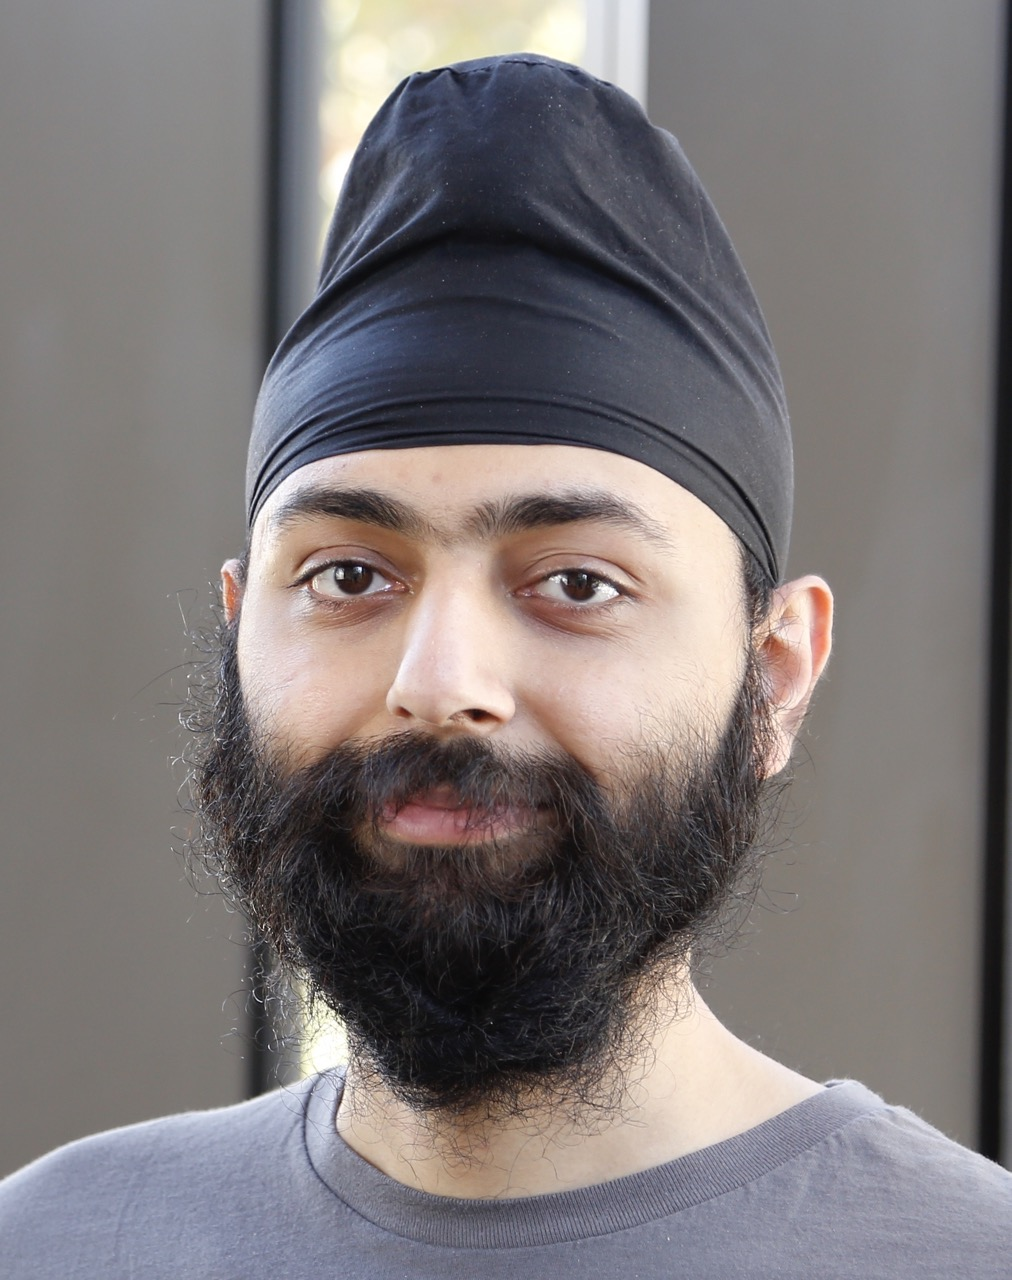
\includegraphics[width=2.2cm]{atul.jpg}
    \end{textblock}

%--------------------SECTIONS-----------------------------------
%Section: Personal Data
\section{Personal}

\begin{tabular}{rl}
    %\textsc{Place and Date of Birth:} & Someplace, Italy  | dd Month 1912 \\
    \textsc{Address:}   & 1318 Cordova St, Pasadena, CA 91106, USA \\
    \textsc{Phone:}     & +1 626 318 0732\\ 
    %\textsc{Mobile:}      
                        & +1 626 515 4073\\
    \textsc{Email:}     & \href{mailto:asarora@caltech.edu}{asarora@caltech.edu}, \href{mailto:atul.singh.arora@gmail.com}{atul.singh.arora@gmail.com}%\href{https://atulsingharora.github.io}{atulsingharora.github.io}
\end{tabular}

%Section: Work Experience at the top

\section{Research Experience}

\begin{longtable}{r|p{11cm}}
  \textsc{2021-}\emph{present}
                   & PostDoc, \textsc{California Institute of Technology}, United States \\
                   &\small Advisor: Prof. Thomas \textsc{Vidick}\\
                  &\footnotesize{Primarily studied hybrid models where depth bounded quantum circuits, can be interleaved with $\BPP$ machines.
                    \begin{itemize}[leftmargin=8pt]
                      \item[] Showed oracle separations among the different hybrid models.\su{1}
                      \item[] Characterised quantum depth, relative to a random oracle.\su{2}
                    \end{itemize}
                    % }
                    % \\
                    % &\footnotesize{~~ End of 2021: Showed oracle separations among the different hybrid models.\su{1}}\\
                    % &\footnotesize{~~ End of 2022: Characterised quantum depth, relative to a random oracle.\su{2}}\\
                    %&\footnotesize{Completed older projects:}\\
                    % &\footnotesize{On the side, worked on quantum foundations and quantum coin flipping.}\\
                    % &\footnotesize{~~ Motivated by contextuality, demonstrated self-testing of a single quantum system (includes both theory and experiment).\su{3}}\\
                    % &\footnotesize{~~ Introduced methods to improve the security of device-independent weak coin flipping protocols, resulting in an improvement after a decade.\su{4}}\\
                    % &\footnotesize{~~ Collected all our previous results on the topic into a journal version---Solutions to Quantum Weak Coin Flipping.\su{5}}\\
                    % &\footnotesize{
                      On the side, worked on quantum foundations and quantum coin flipping.
                    \begin{itemize}[leftmargin=8pt]
                      \item[] Motivated by contextuality, demonstrated self-testing of a single quantum system (includes both theory and experiment).\su{3}
                      \item[] Introduced methods to improve the security of device-independent weak coin flipping protocols, resulting in an improvement after a decade.\su{4}
                      \item[] Solutions to Quantum Weak Coin Flipping---collected all our previous results on the topic into a journal version.\su{5}
                    \end{itemize}
                    } \\
                    % &\footnotesize{Motivated by contextuality, demonstrated self-testing of a single quantum system (includes both theory and experiment).\su{3}} \\
                    % &\footnotesize{Introduced methods to improve the security of device-independent weak coin flipping protocols, resulting in an improvement after a decade.\su{4}}\\ 
                    % &\footnotesize{Collected all our previous results on the topic into a journal version---Solutions to Quantum Weak Coin Flipping.\su{5}}\\

                    &\small{{\tiny $^1$} ASA, A. Gheorghiu, U. Singh. \href{https://arxiv.org/abs/2201.01904}{arXiv:2201.01904} (submitted; \href{https://atulsingharora.github.io/HQC}{web})}\\                                                                     
                    &\small{{\tiny $^2$} ASA, Coladangelo, Coudron, Gheorghiu, Singh, Waldner.  \href{https://arxiv.org/abs/2210.06454}{arXiv:2210.06454}} \\

                    &\small{{\tiny $^3$} X. Hu, Y. Xie, ASA, M. Ai, K. Bharti, et. al. \href{https://arxiv.org/abs/2203.09003}{arXiv:2203.09003} (submitting)}\\  
                    &\small{{\tiny $^4$} ASA, J. Sikora, T Van Himbeeck (submitting; \href{https://www.overleaf.com/read/jhwnvgbntqkd}{overleaf}, \href{http://atulsingharora.github.io/DI_WCF}{web})}\\
                    &\small{{\tiny $^5$} ASA, J. Roland, C. Vlachou, S. Weis. \href{https://eprint.iacr.org/2022/1101}{cryptoeprint:2022/1101} (submitting)}\\
                    %; \href{https://www.overleaf.com/read/khztgjgdgvmm}{overleaf}})\\
  \multicolumn{2}{c}{} \\                   
 \textsc{2016-20}     & PhD Thesis, \textsc{Université libre de Bruxelles (ULB)}, Belgium \\
                    &\emph{Quantum Weak Coin Flipping} \\
                    &\small Advisor: Prof. Jérémie \textsc{Roland}\\
                    &\footnotesize{Primarily worked on quantum weak coin flipping, a cryptographic primitive. Its figure of merit is called the bias, $\epsilon$. The best known had $\epsilon \to 1/6$ by C. Mochon in 2005.
                    \begin{itemize}[leftmargin=8pt]
                      \item[] Protocols with $\epsilon \to 1/10$ were found{\tiny $^1$}.
                      \item[] An algorithm to numerically find protocols with $\epsilon\to 0$ was given{\tiny $^1$}.
                      \item[] An exact (geometric) solution to the problem was found{\tiny $^2$}. 
                      \item[] A simpler, exact (algebraic) solution to the problem was found{\tiny $^3$}.
                    \end{itemize}
                    On the side, investigated foundational aspects of quantum mechanics{\tiny $^4$}. 
                    } \\
                    % &\footnotesize{~~End 2017: Protocols with $\epsilon \to 1/10$ were found{\tiny $^1$}. }\\
                    % &\footnotesize{~~End 2018: An algorithm to numerically find protocols with $\epsilon\to 0$ was given{\tiny $^1$}. }\\
                    % &\footnotesize{~~End 2019: An exact (geometric) solution to the problem was found{\tiny $^2$}. }\\
                    % &\footnotesize{~~Mid 2020: A simpler, exact (algebraic) solution to the problem was found{\tiny $^3$}. }\\
                    % &\footnotesize{On the side, investigated foundational aspects of quantum mechanics{\tiny $^4$}. }\\
                    %&\footnotesize{Current: Simplifying the exact solution. Exploring self-testing using contextuality. Formulating continuous time quantum communication complexity.}\\
                    &\small{{\tiny $^1$}ASA, J. Roland, S. Weis. \href{https://arxiv.org/abs/1811.02984}{arXiv:1811.02984} (\href{https://www.youtube.com/watch?v=eNK6X7BlG5U&list=PLGdMsPGuoD25wLgnY7RBoTAxsnQEMsNA0&index=12}{QIP '19} \href{http://dx.doi.org/10.1145/3313276.3316306}{STOC '19} \href{https://atulsingharora.github.io/WCF}{web}) }\\
                    &\small{{\tiny $^2$}ASA, J. Roland, C. Vlachou. \href{https://arxiv.org/abs/1911.13283v1}{arXiv:1911.13283v1}} (\href{https://atulsingharora.github.io/WCF_2}{web})\\
                    &\small{{\tiny $^3$}ASA, J. Roland, C. Vlachou. \href{https://arxiv.org/abs/1911.13283v2}{arXiv:1911.13283v2} (\href{https://youtu.be/A2GRxspzWUg?t=801}{QCrypt '20} \href{https://youtu.be/nlZ5JhoE0D8}{QIP '21} \href{https://doi.org/10.1137/1.9781611976465.58}{SODA '21} \href{https://atulsingharora.github.io/WCF_2}{web}})\\
                    &\small{{\tiny $^4$}K. Bharti, A.S.A, L. C. Kwek, J. Roland. \href{https://arxiv.org/abs/1811.05294}{arXiv:1811.05294} (\href{https://link.aps.org/doi/10.1103/PhysRevResearch.2.033010}{Phys. Rev. Res. 2, 033010}) }\\
 \multicolumn{2}{c}{} \\

 \textsc{2015-16} & Master's Thesis, \textsc{Indian Institute of Science Education and Research (IISER), Mohali}, India \\
                  &\emph{Contextuality in a Deterministic Quantum Theory}\\
                  &\small Advisor: Prof. Arvind\\ 
                  &\footnotesize{Concluded that contextuality is not a necessary feature of quantum mechanics and proposed an alternative, non functional-consistency, bolstered by an explicit construction.}\\
                  &\small{ASA, K. Bharti, Arvind. \href{https://arxiv.org/abs/1607.03498}{arXiv:1607.03498}; \href{https://doi.org/10.1016/j.physleta.2018.11.049}{Physics Letters A. (Nov 2018)} }\\            
\multicolumn{2}{c}{} \\

\textsc{Summer}   & Internship \textsc{University of Siegen}, Germany\\
2015                  & \emph{Towards a macroscopic test of local realism}\\
                      & \small{Advisor: Prof. Otfried \textsc{Gühne}}\\
                      & \footnotesize{Constructed a Bell inequality using observables bounded in phase space to probe local realism using macroscopic variables.} \\
                      & \small{ASA, A. Asadian. \href{https://arxiv.org/abs/1508.04588}{arXiv:1508.04588}; \href{http://dx.doi.org/10.1103/PhysRevA.92.062107}{Phys. Rev. A 92, 061207} }\\
                      
\multicolumn{2}{c}{} \\

\textsc{2011-14}  & Internships \\
                      &\textsc{IISER Mohali}, India. {\footnotesize Quantum simulation (theory).} 
                      {\footnotesize Advisor:} \small{Prof Arvind}.\\
                      &\textsc{National Physical Laboratory (NPL)}, New Delhi, India. {\footnotesize Set up an experiment to study the dynamics of a dipole lattice.}                    
                      {\footnotesize Advisor:} \small{Dr Ravi \textsc{Mehrotra}}.\\
                      &\textsc{Indian Institute of Technology (IIT), Bombay, India.} {\footnotesize Yarn defect recognition using OpenCV.}  
                      {\footnotesize Advisor:} \small{Prof Anirban \textsc{Guha}}.
\end{longtable}

%Section: Education
\section{Education}
\begin{tabular}{rp{11cm}}	
  \textsc{Sep} 2020 & Doctorat en Sciences de l'ingénieur et technologie,\\
 \textsc{Oct} 2016  & \textbf{Université libre de Bruxelles (ULB)}, Belgium.\\
                    & \\
 \textsc{July} 2016 & Bachelor and Master of Science with \textsc{Physics} major,\\
 \textsc{July} 2011 & \textbf{Indian Institute of Science Education and Research (IISER), Mohali}, India.\\
& CPI: \textbf{9.4} /10. \small Graduated with \emph{rank two.} \\&\\ 
% & Thesis: ``Sublinear and Locally Sublinear Prices'' | \small Advisor: Prof. Erio \textsc{Castagnoli}\\
% &\normalsize \textsc{Gpa}: 28.61/30\hyperlink{grds}{\hfill | \footnotesize Detailed List of Exams}\\&\\
\end{tabular}

\section{Conferences and Seminars}
\begin{longtable}{rrp{11cm}}
  & ~~2022 &\textbf{Poster}. \emph{Oracle separations of hybrid quantum-classical circuits}\\
  &         &Quantum Information Processing (\textsc{QIP}). Caltech, USA\\
  & ~~2022 &\textbf{Poster}. \emph{Improving the security of device independent weak coin flipping protocols.}\\
  &         &Quantum Information Processing (\textsc{QIP}). Caltech, USA\\  
  & ~~2021 &\textbf{Talk}. \emph{Analytic quantum weak coin flipping protocols with arbitrarily small bias}. \\
  &         &ACM-SIAM Symposium on Discrete Algorithms (\textsc{SODA}). Virtual.\\    
  & ~~2021 &\textbf{Invited Seminar}. \emph{Analytic quantum weak coin flipping protocols  $\dots$} \\  
  &        &University of Ottawa (Online). Prof. Broadbent's group.\\
  & ~~2021 &\textbf{Talk}. \emph{Analytic quantum weak coin flipping protocols $\dots$} \\
  &         &Quantum Information Processing (\textsc{QIP}). Online/Munich, Germany.\\  
  & ~~2020 &\textbf{Talk}. \emph{Analytic quantum weak coin flipping protocols $\dots$} \\
  &         &\textsc{QCrypt}. Online/Amsterdam, Netherlands.\\
  & ~2020 &\textbf{Invited Seminar}. \emph{Quantum weak coin flipping} \\
  &         &Perimeter Institute, Canada.\\
  & ~~2019  &\textbf{Participant}. \\
  & ~~~~~~ &\textsc{QuantAlgo} Workshop. CWI, Amsterdam, Netherlands.\\
  & ~~2019 &\textbf{Participant}. \\
  & ~~~~~~ &(Physics) Lindau Nobel Laureate Meeting (\textsc{LiNo}). Lindau, Germany. \\
  & ~~2019 &\textbf{Talk}. \emph{Quantum Weak Coin Flipping}. \\
  & ~~~~~~ &Symposium on Theory of Computing (\textsc{STOC}). Phoenix, Arizona, USA. \\
  & ~~2019 &\textbf{Talk}. \emph{Quantum Weak Coin Flipping}. \\
  & ~~~~~~ &Quantum Information Processing (\textsc{QIP}). University of Colorado, USA. \\
  & ~~2018 &\textbf{Talk}. \emph{Quantum Weak Coin Flipping beyond bias 1/6}. \\  
  & ~~~~~~ &\textsc{QuantAlgo} Workshop. Université Paris-Diderot, Paris, France. \\
  & ~~2018 &\textbf{Poster}. \emph{Quantum Weak Coin Flipping with bias 1/10}. \\
  & ~~~~~~ &Quantum Information Processing (\textsc{QIP}). TU Delft, Netherlands. \\
  & ~~2017 &\textbf{Participant}. \\
  & ~~~~~~ &Theory of Quantum Computation, Communication and Cryptography (\textsc{TQC}). Paris, France.
  \end{longtable}

%Section: Scholarships and additional info
\section{Recognition }
\begin{tabular}{rrp{11cm}}
  & ~~2020 & \emph{IQIM Postdoctoral Scholarship}, California Institute of Technology. \\
  & ~~2020 & Offered. \emph{Hartree Postdoctoral Fellowship}, University of Maryland.\\  
  & ~~2019 & Granted financial support for attending the \emph{(Physics) Lindau Nobel Laureate Meeting, 2019}. \\
  & ~~2018 & Renewed. Two year research fellowship from the Belgian \emph{Fonds National Recherche de Science (FNRS)}, through the FRIA grant.\normalsize\\
  & ~~2016 & Awarded. Two year research fellowship from the Belgian \emph{Fonds National Recherche de Science (FNRS)}, through the FRIA grant.\normalsize\\
 & ~~2016     & Top 5\% in the physics stream of the \emph{Graduate Aptitude Test in Engineering (GATE)}, India. \\
 & ~~~~~~     & Obtained a 92.3 percentile in the national graduate physics exam, \emph{Joint Entrance Screening Test (JEST)}, India. \\
% \end{tabular}

% \begin{tabular}{rp{11cm}}
 & ~~2015     & Awarded the \emph{Junior Research Fellowship (JRF-NET)} from the Council of Scientific and Industrial Research, India. \\
 & ~~~~~~     & Awarded the \emph{DAAD WISE} fellowship for a summer internship by and in Germany.\\
 & 2013-16  & Awarded the Certificate of Merit for the best academic performance in a semester, twice by IISER. Was among the highest scorers four other times.\\
 & ~~2012     & Awarded the \emph{KVPY} fellowship for my work on Stepper Motor Control, by DST, India.\\
 & ~~2010     & Granted financial support for attending the Bright Green Youth climate summit, Denmark.
\end{tabular}


  \section{Teaching}
  \begin{tabular}{rrp{11cm}}
  & ~~2022 &Tutor. Week-long graduate school on post-quantum cryptography. IPAM, UCLA.\\
  & ~~2019 &Teaching Assistant. Information Quantique (graduate). ULB, Brussels.\\  
  & ~~2016 &Teaching Assistant. Thermodynamics (undergraduate). IISER, Mohali.\\
  & ~~2015 &Teaching Assistant. Classical Mechanics (undergraduate). IISER, Mohali.
  \end{tabular}

  \section{Review}
  Reviewed articles for the following conferences/journals.\\
  \begin{tabular}{rrp{11cm}}
    & ~~2022 & MFCS, JACM and QIP\\
    & ~~2021 & QCrypt\\
    & ~~2019 & QIP, STOC\\
    \end{tabular}
  


%Section: Languages
\section{Languages}
\begin{tabular}{rl}
\textsc{English:}&Fluent\\
\textsc{Hindi:}&Fluent\\
\textsc{French:}&Intermediate\\
\textsc{Punjabi:}&Intermediate\\
\textsc{German:}&Beginner\\
\end{tabular}


% \section{Computer Skills}
% \begin{tabular}{rl}
%  Basic Knowledge:& \textsc{php}, my\textsc{sql}, \textsc{html}, Access, \textsc{Linux}, ubuntu, {\fb \LaTeX}\setmainfont[SmallCapsFont=Fontin-SmallCaps.otf]{Fontin.otf}\\
% Intermediate Knowledge:& \textsc{vba}, Excel, Word, PowerPoint\\
% \end{tabular}

\section{Interests \& Extracurricular}
Technology, Open-Source, Programming (C/C++, Python, Fortran, Javascript);\\ 
Philosophy, Reading; \\
Fitness; Piano, Guitar, Violin.
% \section{Extracurricular}

% \textsc{\href{https://qlic-meets.github.io}{QLIC-meets}} --- \emph{Organizer.} {\footnotesize Department meetings/lectures held to facilitate collaboration. Status: Running. } \\
% \textsc{\href{https://c-est-ca.github.io}{C'est ça}} --- \emph{Editor.} {\footnotesize An at least bilingual peer-reviewed popular science journal. Status: Initialising. }\\
% \textsc{\href{https://gleaned.github.io}{gleaned}} --- \emph{Author.} {\footnotesize Collection of my book summaries. Status: Pilot.}\\
%\textsc{\href{https://donkeydocs.github.io}{donkeyDocs}} --- \emph{Contributor.} {\footnotesize A repository of lecture notes. Status: Initialising. }\\

% \newpage
% \par{\centering\Large \hypertarget{grds}{Bachelor and Master of Science with a major in \textsc{Physics}}\par}\normalsize
% \setlength{\extrarowheight}{7pt}

% \begin{center}
% \label{grades}
% \begin{tabular}{cp{9cm}c}
%   \textsc{Semester$^*$} & \multicolumn{1}{c}{\textsc{Subjects}} & \textsc{Score} \\
%   \hline
%   1 & Mechanics, Chemistry of elements and chemical transformations, 
%   Cellular basis of life, Symmetry, Language skills B (English), 
%   Introduction to computers, Physics lab I, Chemistry lab I, Biology lab I &8.5/10 \\
%   2 & Electromagnetism, Atoms molecules and symmetry, Gene expression and development, Analysis in one variable,
%   Hands-on electronics, History of science, Physics lab II, Chemistry lab II, Biology lab II &8.6/10 \\
%   3 & Waves and optics, Spectroscopic and other physical methods, Genetics and evolution, Curves and surfaces, 
%   Introduction to astrophysics, Workshop training, Physics lab III, Chemistry lab III, Biology lab III &8.8/10\\
%   4 & Thermodynamics and statistical physics, Energetics and dynamics of chemical reactions, Behaviour and ecology,
%   Probability and statistics, Introduction to quantum physics, Philosophy of science, Physics lab IV, Chemistry lab IV,
%   Biology lab IV& 9.7/10 \\
%   5$^\dagger$ & Classical mechanics, Quantum mechanics, Electrodynamics, Advanced optics lab, Reason and rationality & 10/10\\
%   6 & Statistical mechanics, Atomic and molecular physics, Quantum computation, Advanced electronics and instrumentation
%   lab, Quantum field theory & 9.6/10 \\
%   7 & Solid state physics, Nuclear and particle physics, Nuclear physics lab, Physics of fluids, Quantum principles 
%   and quantum optics, Radiative effects and renormalisation group in relativistic quantum field theory & 9.4/10\\
%   8 & Nonlinear dynamics, Chaos and complex systems, Condensed matter physics lab, computational methods in physics,
%   Standard model and beyond, Selected topics in classical and quantum mechanics& 9.5/10\\
%   9 & Ethics, MS Thesis---Research project I & 10/10 \\
%   10 & Cosmology and galaxy formation, MS Thesis---Research project II & 10/10\\
%   & \cline{2-2}
%   &Cumulative Performance Index (CPI)& \textbf{9.4} /10\\
%   & \\
%   \hline
% \end{tabular}
% \end{center}
% \vspace*{\fill}
% \hrule
% \footnotesize{$*$ Note that the credits associated with each semester are not exactly the same.}

% \footnotesize{$\dagger$ Physics major henceforth.}



%\newpage
%\hypertarget{gmat}{\textsc{Gmat}\setmainfont{LMRoman10 Regular}\textregistered\setmainfont[SmallCapsFont=Fontin-SmallCaps]{Fontin-Regular}}

%\XeTeXpdffile ''GMAT.pdf'' page 1 scaled 800

\end{document}
